\tikzsetnextfilename{externalized-gps_test_setup}
 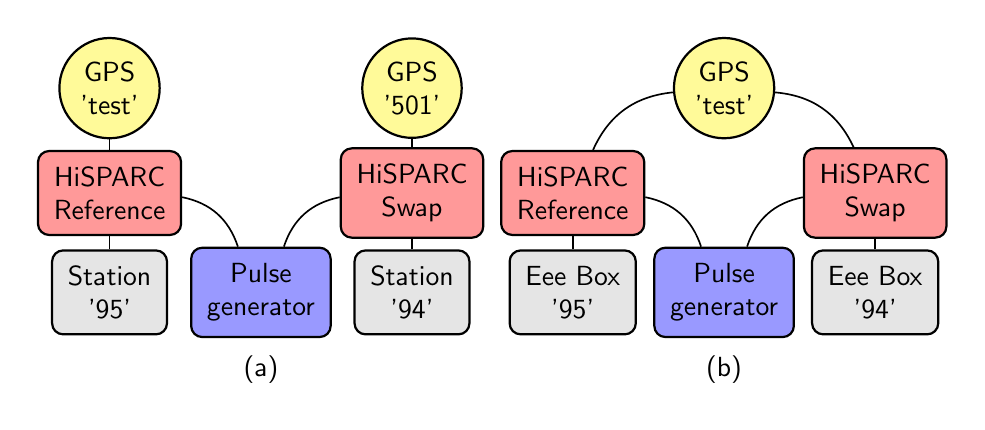
\begin{tikzpicture}
  [font=\sffamily,
   every matrix/.style={ampersand replacement=\&,column sep=0.1cm,row sep=0.1cm},
   gps/.style={draw,thick,circle,fill=yellow!40,inner sep=.1cm, align=center},
   pc/.style={draw,thick,rounded corners,fill=black!10,inner sep=.2cm, align=center},
   hisparc/.style={draw,thick,rounded corners,fill=red!40,inner sep=.2cm, align=center},
   pulse/.style={draw,thick,rounded corners,fill=blue!40,inner sep=.2cm, align=center},
   to/.style={-,semithick,font=\sffamily\footnotesize},]

  \matrix{
   \node[gps] (test) {GPS\\'test'}; \& \& \node[gps] (501) {GPS\\'501'}; \& \& \& \node[gps] (b_test) {GPS\\'test'}; \& \\
   \node[hisparc] (refr) {HiSPARC\\Reference}; \& \& \node[hisparc] (swap) {HiSPARC\\Swap}; \& \& \node[hisparc] (b_refr) {HiSPARC\\Reference}; \& \& \node[hisparc] (b_swap) {HiSPARC\\Swap}; \\
   \node[pc] (95) {Station\\'95'}; \& \node[pulse] (pulse) {Pulse\\generator}; \& \node[pc] (94) {Station\\'94'}; \& \& \node[pc] (b_95) {Eee Box\\'95'};  \& \node[pulse] (b_pulse) {Pulse\\generator}; \& \node[pc] (b_94) {Eee Box\\'94'}; \\
   \& \node {(a)}; \& \& \& \& \node {(b)}; \& \\
  };
  
  \draw[to] (test) -- node[below,above,sloped] {} (refr);
  \draw[to] (501) -- node[below,above,sloped] {} (swap);
  \draw[to] (95) -- node[midway,midway,sloped] {} (refr);
  \draw[to] (94) -- node[midway,midway,sloped] {} (swap);
  \draw[to] (pulse) to[bend left] node[above,below,sloped] {} (swap);
  \draw[to] (pulse) to[bend right] node[above,below,sloped] {} (refr);

  \draw[to] (b_test) to[bend right] node[below,above,sloped] {} (b_refr);
  \draw[to] (b_test) to[bend left] node[below,above,sloped] {} (b_swap);
  \draw[to] (b_95) -- node[midway,midway,sloped] {} (b_refr);
  \draw[to] (b_94) -- node[midway,midway,sloped] {} (b_swap);
  \draw[to] (b_pulse) to[bend left] node[above,below,sloped] {} (b_swap);
  \draw[to] (b_pulse) to[bend right] node[above,below,sloped] {} (b_refr);

 \end{tikzpicture}
